\documentclass[12pt]{article}%
\usepackage{hyperref}
\usepackage{graphicx}

\begin{document}

\title{CS472 Assignment 2}
\author{Mark Bereza}
\date{\today}
\maketitle
\section{Part 1}
For Part 1, I first looked at the man page for frexp() and ran it with the test code snippet provided. I then aimed to created a function that would produce exactly the same output regardless of what double was provided. I calculated/looked up the number of bits, the appropriate mask, and the required bit shifts for each portion of an IEEE double and defined macros for each. For normal values, I noticed that frexp() simply prints the fraction with the sign expressed as a value between 0.5 and 1. Since the actual mantissa is always a value between 1 and 2, I simply extracted the mantissa bits, added the leading 1, and divided by 2. To account for this, I also incremented the exponent. For infinite and NaN values, frexp() simply returned the input value as the fraction and 0 as the expoonent, so I made a branch that does exactly that. Finally, I handled denormal values by making sure to not add the leading one and simply multiplying the mantissa by 2 (and decrementing the exponent) until I got a fraction that was between 0.5 and 1.

To demonstate that it works, I created an array of test values, including every edge case I could think of and ran both frexp() and my_frexp() on each, printing the results side by side. I verified that they were identical.
\section{Part 2}
\subsection{Software Floating Point Operations Implementation}
For Part 2, I started by defining my own bitfield (54 bits in size) that would store data exactly the same way a regular double does and named it my_double. To make my life easier, I also defined constants for the my_double versions of NaN and zero and also defined functions to convert doubles and unsigned 64-bit ints to/from my_doubles. The former would make printing my_doubles possible and the latter would allow me to easily create my_doubles out of bit patterns.
\subsubsection{Addition}
For addition, I simply made the operand of larger magnitude the first one, shifted the second's mantissa right until the exponents matched, and added the mantissa's together. I accounted for overflow by right-shifting once and incrementing the exponent. I also made some branches to account for operations that could produce inf or NaN.
\subsubsection{Subtraction}
For this, simply flipped the sign of subtrahend and then performed addition on the two operands.
\subsubsection{Multiplication}
Since I knew that I would have to multiply the mantissas together and that multiplication of two 52-bit values could overflow a 64-bit unsigned integer, I adapted \hyperref[John Hauser's Berkeley SoftFloat]{''http://www.jhauser.us/arithmetic/SoftFloat.html''} algorithm for multiplying two 64-bit ints and storing the result in a 128-bit struct. From there, I simply shifted left or right until the resulting mantissa was between 1 and 2, added the exponents, and applied decrements/increments based on the number of times the resulting mantissa needed to be shifted. As with addition/subtraction, I also put in caveats to catch operations that should produce inf or NaN.
\subsubsection{Division}
For division, I simply implemented \hyperref[Newton-Raphson division]{''https://en.wikipedia.org/wiki/Division_algorithm#Pseudocode''}, making sure to use my version of floating point subtraction and multiplication during the intermediate steps. To efficiently use the constants the algorithm calls for (48/17 and 32/17), I determined the bit pattern for the IEEE double precision floating point representation of these values and stored said bit patterns as macros, converting them in my_doubles as needed. As before, I added branches to handle edge cases like division by zero and others.
\subsubsection{Square Root}
For square root, I decided to use the fast software floating point inverse square root function used in the \hyperref[Quake III source]{https://github.com/id-Software/Quake-III-Arena/blob/master/code/game/q_math.c#L552}. I adapted it from single-precision to double-precision floats by changing the magic number used from 0x5f3759df to 0x5FE6EB50C7B537A9 and by increasing the number of iterations of Newton's method from one to three to accomodate for the increased precision of doubles. Finally, I multiplied the result by the radicand to convert from the inverse square root to a regular square root. I also ensured that trying to perform the operation on any negative value would return NaN.
\subsubsection{Testing Accuracy}
To make sure my floating point operations were actually returning the correct results, I created a program that would take two operands as command line arguments and perform each of the five arithmetic operations on them and print the results. I ran these on a large number of test cases and checked the results against a calculator. I did not test operations that should result in denormal values since I never handling for those cases.
\subsection{Operation Timing and Comparison}
To time how long it takes to perform each of the five arithmetic operations in both software and hardware, I decided to use getrusage() since it conveniently only times how long code actually runs on the CPU, avoiding inaccuracy or bias resulting from context switching during execution. I followed the methodology described in class to get a timing value large enough to measure and to isolate the computation of the operations from the for loop overhead. That is, I ran 40x of each operation thousands of times, subtracted the time it took to run 20x of the same operation thousands of time and divided the resulting time by the number of total operations ran, with the results being in realm of nanoseconds. After running my code 10 times, I averaged the results and stored them in a table, displayed below:\\ \\
\begin{minipage}{\linewidth}
\begin{center}
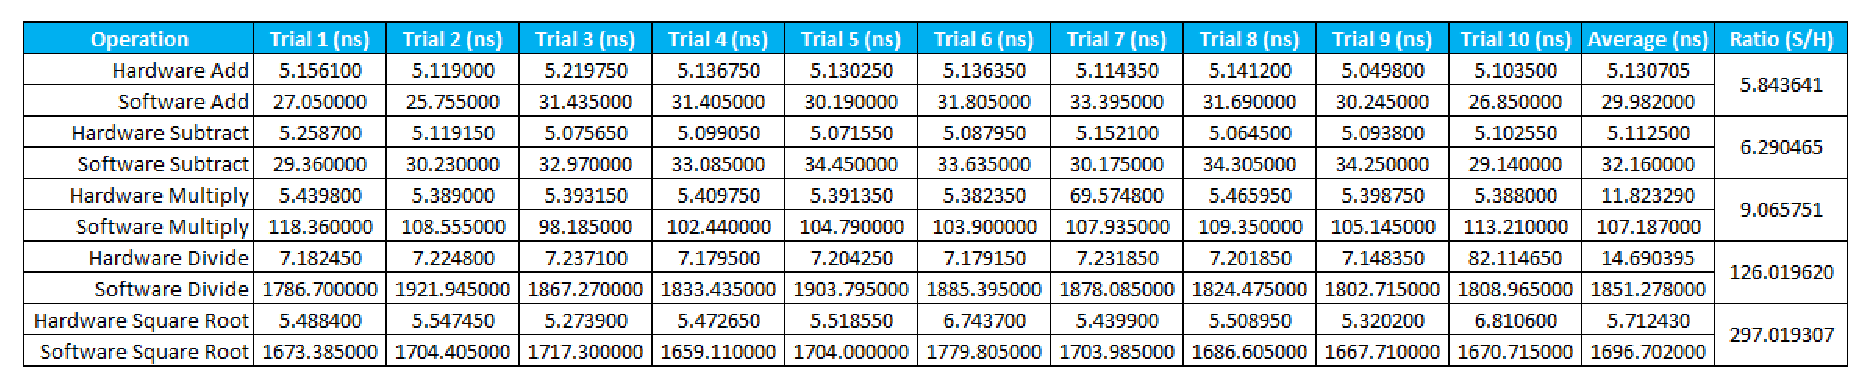
\includegraphics[width=0.8\textwidth]{timing_data.eps}
\captionof{figure}{Spreadsheet of timing data for software/hardware implementations of floating point operations. The final column shows many times faster the hardware version is than the software version for each of the five operations.}
\end{center}
\end{minipage}
\\Unsurprisingly, the hardware versions are significantly faster, ranging from ~10 times faster for simple operations like addition, subtraction, and multiplication to hundreds of times faster for complex multi-step operations division and square root.
\section{Part 3}
For this part, I simply created a union that held a unsinged 64-bit int (for the bits), a double, a long, and an 8-character array. I randomly generated a 64-bit value using the 64-bit version of the Mersenne Twister and interpreted the bits as each of the different values, printing the results for each.
\end{document}
